\section{Minería de Texto}
\lhead[\thepage]{\thesection Minería de Texto}

\subsection{Definición}
  En ``Untangling Text Data Mining'' , Hearst describe la minería de texto como una extensión natural de la minería de datos, cuyo objetivo principal es descubrir nuevos conocimientos e información, enfatiza la diferencia que existe entre esta y la minería de datos, en donde la búsqueda de patrones y tendencias se realiza generalmente con el objetivo de apoyar la toma de decisiones mas que el de descubrir información y conocimientos novedosos, esto ultimo lo considera algo mas propio del campo de la minería de texto. Esto se resume en la comparación hecha en el Cuadro \ref{tab:comphearst} por Hearst. \cite{untangling}
  

	 \begin{table}[ht]
      \centering\scriptsize
      \begin{tabular}{|c|c|c|c|c|c|}
       \hline 
        & Encontrando Patrones & \multicolumn{2}{ c| }{ Encontrando Nuggets}\\ \cline{1-4}
        & & Novedoso & No-Novedoso\\ \cline{1-4}
       Datos no-textuales & Mineria de datos estandar & ? & Consultas a base de datos \\ \cline{1-4}
       Datos textuales & lingüistica computacional & Minería de texto real & Recuperación de información\\ \cline{1-4}
      \end{tabular}
      \caption{Clasificación de aplicaciones de la minería de texto y minería de datos}
       \source{http://people.ischool.berkeley.edu/\~hearst/papers/acl99/acl99-tdm.html}
      \label{tab:comphearst}
  \end{table}
 

  En obras mas modernas vemos que la definición toma un aspecto general. La minería de texto puede ser definida como un proceso
  en el que un usuario interactúa con una colección de documentos usando un conjunto de herramientas de análisis, resaltando que la fuente de datos utilizada en minería de texto no son bases de datos estructuradas, sino datos textuales no estructurados en los documentos que forman parte de la colección analizada.\cite{tmhandbook}

  Puede así definirse la minería de texto como un proceso de análisis aplicado sobre datos textuales no estructurados contenidos en una colección de documentos, para el descubrimiento de información no descrita de forma explicita en los documentos analizados.

\subsection{Conceptos Básicos}

  \subsubsection{Colección de documentos}
    Cualquier agrupación de documentos de texto. Pueden ser estáticos, en cuyo caso el grupo inicial de documentos no cambia, o dinámicos termino que aplica a colecciones donde los documentos son actualizados o se agreguen nuevos documentos gradualmente.\cite{tmhandbook}

  \subsubsection{Documento}
    Puede definirse informalmente como una unidad discretas de datos textuales en una colección, que usualmente, pero no necesariamente, esta correlacionado con un documento del mundo real, como un memorandum legal, e-mail, articulo,  entre otros. Se debe resaltar que un documento no existe en una única colección, puede ser parte de cualquier numero de colecciones.\cite{tmhandbook}


  \subsubsection{Pre-procesamiento}
    Esta fase de la minería de texto (y la minería de datos) busca la conversión de los datos no estructurados y semi-estructurados a una representación estructurada como lo es un modelo vectorial. Esta fase debe llevarse acabo antes de realizar cualquier tarea de análisis o de minería de texto avanzada. Los pasos posibles de pre-procesamiento son los mismos en toda tarea de minería de texto, sin embargo cuales pasos son escogidos dependerán de la tarea a realizar.\cite{txtMiningGaryMiner}  % gary miner, practical text mining and statistical analysis for non structured text data https://books.google.co.ve/books?id=SM94BMsy50gC&printsec=frontcover&hl=es#v=onepage&q&f=false
    Los pasos básicos para el pre-procesamiento son los siguientes:
    \begin{itemize}
        \item Escoger el alcance de los textos ( \textit{Scope of documents} ): Esta etapa busca determinar si se usaran documentos completos, secciones, párrafos, u otras divisiones posibles de un documento para su posterior procesamiento usando técnicas de minería de texto. La decisión tomada dependerá del objetivo de la tarea de minería de texto, por ejemplo para tareas relacionadas con \textit{ e-mails } se escogerían los correos como el alcance, en documentos grandes esta tarea puede dificultarse, generalmente para análisis que involucren clasificación o agrupación se toma cada documento entero como el alcance.\cite{txtMiningGaryMiner}
        \item Tokenización ( \textit{Tokenization} ): Consiste en dividir las unidades de texto en palabras individuales llamadas \textit{tokens}. Esta tarea es dependiente del lenguaje en el que se encuentren los documentos, para lenguajes como el español o el ingles, una estrategia común es tomar los \textit{tokens} entre espacios o signos de puntuación, sin embargo este método debe lidiar con casos como las abreviaciones. Se puede lidiar con esta clase de inconvenientes usando métodos de tokenización inteligente que reconocen estos casos especiales.\cite{txtMiningGaryMiner}
    \item Remover palabras no informativas ( \textit{Stopping} ): en muchos casos de análisis con minería de texto es útil remover palabras comunes cuya aparición ocurre en la mayoría de textos, tales como los artículos o conectivos. Estas palabras son conocidas como \textit{stopwords} y el proceso de eliminarlas como \textit{stopping}. La remoción de estas palabras no tiene un impacto significativo en gran parte de los casos de minería de texto debido a que en los algoritmos y tecnicas usadas las \textit{stopwords} tienen poco o ningún impacto en los resultados finales. Sin embargo en casos como la recuperación de información \textit{information retrieval} el \textit{stopping} es contraproducente ya que las frases pierden su significado si algunas palabras son removidas.\cite{txtMiningGaryMiner}

    \item \textit{Stemming} y Lematización (\textit{Lemmatization}) :  \textit{stemming} es el proceso de normalizar palabras relacionadas a una misma forma. Este proceso incluye la identificación y eliminación de prefijos, sufijos y pluralizaciones inapropiadas hasta obtener un \textit{token} general que identifique todas las palabras que esten relacionadas. Como efecto de este proceso se reduce la dimensionalidad mejorando el desempeño de los algoritmos. La lematización es una forma avanzada de \textit{stemming} que intenta agrupar palabras basándose en su núcleo o lemma, el cual es determinado a partir del análisis del contexto que rodea a la palabra e información gramatical.\cite{txtMiningGaryMiner}


    \end{itemize}

  \subsubsection{Características del documento}
    La etapa de pre-procesamiento intenta aprovechar los diferentes elementos contenidos en el lenguaje natural de un documento, para transformarlo de una estructura implícita e irregular a una representación explicita. Sin embargo debido al numero de elementos que contiene un documento se debe poner especial énfasis durante el proceso de minería de datos en la identificación de un conjunto simplificado de elementos que representen al documento por completo, este conjunto de características se conoce como el modelo representativo del documento.\cite{tmhandbook}

    Debido a que los algoritmos para minería de texto operan sobre representaciones del documento basadas en características, existe una negociación entre dos metas importantes. La primera meta es representar de una forma precisa el significado del documento, lo que se traduce en un aumento de sus características representativas.
    La segunda meta es identificar las características de tal forma que sean lo mas computacionalmente eficientes y practicas para el descubrimiento de patrones, que es un proceso que busca la simplificación de los conjuntos de características.\cite{tmhandbook}

    Aunque son muchas la características que pueden representar un documento las siguientes cuatro son las mas usadas para este propósito:

    \begin{itemize}
    \item Caracteres: Los componentes individuales como letras, números, caracteres especiales y espacios son la unidad básica de construcción de características de alto nivel semántico como palabras, términos y conceptos.\cite{tmhandbook}

    \item Palabras: son el nivel básico que presenta un valor semántico. En general una característica de este nivel equivale o tiene el valor de un toquen lingüístico.  Frases, expresiones con múltiples palabras o incluso palabras unidas con guion, no constituyen características del nivel de una palabra.\cite{tmhandbook}
    \item Términos: son palabras y frases seleccionadas directamente del corpus de un documento por medio de metodologías de extracción de términos. Características de este nivel pueden estar conformadas unicamente por expresiones y palabras especificas encontradas en el documento para el que son representativas.\cite{tmhandbook}

    \item Conceptos: son características generadas para un documento por medio de metodologías de categorización manual, estadística, basa en reglas o híbridas. Pueden estar conformadas por palabras, expresiones, clausulas completas o inclusive unidades sintácticas mas grandes. Muchas de las metodologías usadas involucran un grado de referencias cruzadas con fuentes de conocimiento externo. A diferencia de las características basadas en palabras o términos, las características al nivel de conceptos pueden consistir de palabras que no estén específicamente en el documento nativo.\cite{tmhandbook}
    \end{itemize}

\subsection{TF-IDF}
  TF-IDF es un esquema de ponderación que va mas alla de evaluar si una palabra aparece o no en un documento, combina dos definiciones TF e IDF. 
  La frecuenta de términos (TF por su nombre en ingles \textit{Term Frequency}) consiste en asignar a un termino perteneciente a un documento un peso igual al numero de ocurrencias del mismo en dicho documento, se denota como $tf(t,d)$  donde $t$ representa al termino y $d$ al documento. Este método de ponderación sufre de una deficiencia, todos los términos son considerados con la misma importancia al evaluarse su relevancia para una consulta, cuando de hecho algunos términos tienen poco o ningún poder al determinar la relevancia. \cite{informationretrieval}

  IDF (por su nombre en ingles \textit{Inverse Document Frequency}) surge como una medida de contrapeso para la deficiencia de TF mencionada en el párrafo anterior. Consiste en atenuar el efecto de aquellos términos con una ocurrencia muy frecuente en la colección como para ser considerados en la determinación de la relevancia. Para este fin se denota el numero de documentos en la colección que contienen al termino $t$ como la frecuencia del documento $df_t$, y el numero total de documentos en la colección como $N$, se define entonces la frecuencia inversa del documento (idf) de un termino $t$ como sigue:
  
  \begin{equation} \label{eq:idf} 
idf_t=\log\frac{N}{df_t}
\end{equation}


  De esta forma el factor IDF es calculado con el objetivo de escalar la ponderación del termino de tal forma que el $idf$ de un termino raro es alto, mientras que el $idf$ para un termino frecuente es mas probable que sea bajo. 

  Las dos definiciones básicas TF e IDF son combinadas para producir el esquema de ponderación TF-IDF donde a cada termino $t$ le es asignado un peso en el documento $d$, esto viene dado por:
  \begin{equation} \label{eq:tfidf} 
tf\mathrm{-}idf(t,d)=tf_{t,d}\times idf_t
\end{equation}

  Esta ponderación cuenta con las siguientes características: 
  \begin{itemize}
    \item Es mayor cuando $t$ ocurre gran cantidad de veces en un numero pequeño de documentos.
    \item Menor cuando el termino ocurre pocas veces en un documento, o ocurre en muchos documentos.
    \item Mucho menor cuando el termino ocurre prácticamente en todos los documentos.
  \end{itemize}

\subsection{El modelo espacio vector y la matriz de término-documento}

  Usando el método de ponderación TF-IDF, se visualiza cada documento como un vector con una componente para cada termino contenido en la colección (este conjunto de términos es conocido como diccionario de términos, o simplemente diccionario)  junto a la ponderación dada por TF-IDF. Para términos que no ocurran en un documento su ponderación es cero.\cite{informationretrieval} 

  Esta representación del conjunto de documentos como vectores en un espacio vectorial común, es conocida como el modelo espacio vector.\cite{informationretrieval}

  Al verse un conjunto de $N$ documentos como una colección de vectores, entonces se tiene lo que es conocido como la matriz de término-documento esta es una matriz $M\times N$ cuyas filas representan los $M$ terminos de las $N$ columnas, cada una de las cuales corresponden a un documento.\cite{informationretrieval}

\subsection{Medidas de similitud entre vectores}
  Habiéndose planteado la representación de los documentos como vectores, un elemento clave para operaciones de clasificación y agrupamiento es encontrar la similitud entre dichos vectores (y por tanto entre los documentos). Con este fin se presentan las ecuaciones mas utilizadas para obtener una ponderación de la similitud:
  \subsubsection{Distancia euclídea}
    Métrica estándar para problemas geométricos, es la distancia ordinaria entre dos puntos en el espacio.
    Dados dos documentos $d_1$ y $d_2$ representados vectorialmente. La distancia euclídea entre dos documentos viene dada por:  
    \begin{equation} \label{eq:deuc} 
D(d_1,s_2)=\sqrt{\sum\limits_{i=0}^n {|d_{1,i}-d_{2,i}|}^2 }
\end{equation}

  \subsubsection{Similitud del coseno}
    Al ser representados los documentos como vectores es posible usar la correlación que existe entre ellos, siendo dos vectores $d_1$ y $d_2$ para conocer la similitud entre estos puede usarse el coseno del angulo que existe entre dicho vectores.

    Esta medida viene dada por la siguiente ecuación: 
    \begin{equation} \label{eq:cos} 
Cos(d_1,d_2)=\frac{d_1\cdot d_2}{||d_1||\cdot ||d_2||}
\end{equation}

    Donde es normalizada con la distancia euclídea ($||\cdot||_2$).

\subsection{Algoritmos de agrupación (\textit{clustering})}
  Los algoritmos de \textit{clustering} agrupan un conjunto de documento en subconjuntos o \textit{clusters}. En estos algoritmos se busca crear \textit{clusters} que posean una coherencia interna, pero estén bien diferenciados entre ellos. Son las características y distribución de los datos lo que determina la correspondencia de un documento a un grupo, no existe asignación previa de clases por lo que la agrupación es la forma mas común de aprendizaje no supervisado.
  
  
  Pueden distinguirse dos tipos de agrupamiento; agrupamiento plano (\textit{Flat clustering}), en donde el conjunto de \textit{clusters} no posee ninguna estructura explicita que relacione las agrupaciones entre ellas, agrupaciones jerárquicas (\textit{Hierarchical clustering}), en donde se crea una jerarquía entre los agrupamientos que conforman el conjunto de  \textit{clusters}.\cite{informationretrieval}
  
  El objetivo en \textit{Flat clustering} es que dado un conjunto de documentos $D = \{d_1,...,d_N\}$, el numero deseado de \textit{clusters} $K$, y una función objetivo que evalué la calidad de la asignación a las diferentes agrupaciones, se desea computar una asignación $\gamma:D\to\{1,...,K\}$ que minimice (o en otros casos maximice) la función objetivo. En la mayoría de los casos también se demanda que ninguna agrupación $K$ este vacía.\cite{informationretrieval}

  La función objetivo es generalmente definida en términos de similitud o distancia entre documentos. La selección del numero $K$ usualmente no es mas que una buena aproximación basada en experiencia o dominio de conocimiento. Sin embargo existen una serie de heuristicas que se pueden seguir para encontrar un numero adecuado de particiones, estas heuristicas se detallaran mas adelante. Otro problema que se discutirá surge de encontrar puntos de inicios adecuados, ya que si se escogen de forma desfavorable se puede perder el optimo global.\cite{informationretrieval}

    
  \subsubsection{K-medias (\textit{K-means})}
    Es uno de los algoritmos mas importantes de agrupamiento, pertenece a la categoría de agrupamiento plano, tiene como objetivo minimizar el promedio de la distancia euclídea cuadrada de documentos a partir de los centros de sus agrupaciones (\textit{clusters}), donde el centro de una agrupación se define como la media o centroide $\vec{\mu}$ de los documentos en una agrupación $\omega$: 
    \begin{equation} \label{eq:centroide} 
\vec{\mu}= \frac{1}{|\omega|}\sum_{\vec{x}\in\omega}\vec{x}
\end{equation} 
 

    Esta definición se hace en base a el modelo de espacio vector, planteado anteriormente. Una agrupación ideal en K-medias es una esfera con un centroide como su centro de gravedad. Idealmente, las agrupaciones no deben superponerse.\cite{informationretrieval}

    Una medida de evaluar que tan bien los centroides representan a los miembros de sus agrupaciones es la suma residual de cuadrados, $RSS$ (por su nombre en ingles \textit{residual sum of squares}), la distancia cuadrada de cada vector desde su centroide sumada sobre todos los vectores, esto es:
    \begin{equation} \label{eq:RSSk} 
RSS_k=\sum_{\vec{x}\in\omega_k}|\vec{x}-|\vec{\mu}(\omega_k)|^2
\end{equation}


    \begin{equation} \label{eq:RSS} 
RSS=\sum_{K=1}^k{RSS_k}
\end{equation}

    El objetivo en K-medias es minimizar a RSS.

    \begin{figure}[!htbp]
      \centering
      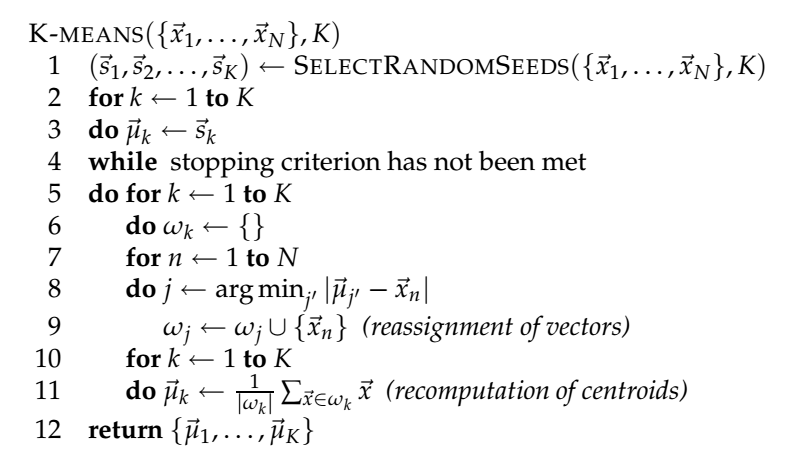
\includegraphics[width=0.7\textwidth]{Figuras/codigo_kmedias.png}
      \caption{Pseudocodigo del algoritmo de k-medias}
      \label{fig:cod_kmedias}
      \source{Imagen extraída de \cite{informationretrieval}}
   \end{figure}

    
    En base a la figura \ref{fig:cod_kmedias} se describe el algoritmo de k-medias de forma general en los siguientes pasos, se seleccionan $K$ documentos de forma aleatoria como centros iniciales de los \textit{clusters}, conocidos como semillas (\textit{seeds}). Dichos centros son transladados en el espacio, con el objetivo de minimizar RSS. Esto se hace de forma iterativa hasta cumplir con un criterio de parada, reasignando documentos al \textit{cluster} con el centroide mas cercano y recalculando cada centroide basado en los miembros actuales de su \textit{cluster}.\cite{informationretrieval}
    
    
    Los criterios de parada aplicables son:
      \begin{itemize}
        \item Un numero fijo de iteración, si bien esta condición limita el tiempo de ejecución del algoritmo puede provocar una calidad baja de agrupamiento debido a un numero insuficiente de iteraciones.
        \item La asignación de los documentos a los \textit{clusters} no cambia, exceptuando casos con malos mínimos locales. Este criterio produce una buena asignación a los \textit{clusters} pero el tiempo de ejecución podría ser excederse del rango aceptable.
        \item Los centroides no cambian entre iteraciones.
        \item Detener la ejecución del algoritmo cuando $RSS$ caiga debajo de un rango. Este criterio asegura que las agrupaciones sean de una calidad deseado al terminar el proceso. Se combina con un numero de iteraciones máximas para asegurar que la ejecución acabe.
        \item Detener la ejecución del algoritmo cuando el descenso en $RSS$ caiga debajo de un rango $\theta$. Este criterio asegura que las agrupaciones sean de una calidad deseado al terminar el proceso. Se combina con un numero de iteraciones máximas para asegurar que la ejecución acabe.
      \end{itemize}
    
    \paragraph{Cardinalidad de \textit{clusters} en K-medias}

    Seleccionar un $K$ adecuado es uno de los factores fundamentales para obtener resultados adecuados al usar K-medias, existen diferentes criterios a los que recurrir si no se puede estimar de forma previa un valor adecuado para $K$.\cite{informationretrieval}

    Un método heuristico para estimar un $K$ que minimice a $RSS$ es ejecutar $i$ agrupamientos con $K$ \textit{clusters} (cada uno con una inicialización diferente) y calcular la función $RSS$ de cada uno de estos. Luego es tomado el mínimo de los valores $RSS$ de los $i$ agrupamientos. Este mínimo es denotado como $RSS_{min}(K)$. Mientras $K$ es incrementado se inspeccionas los valores de $RSS_{min}(K)$ hasta encontrar el `codo' en la curva, este es el punto donde el decrecimiento sucesivo en $RSS_{min}(K)$ se hace notablemente pequeño. Ejemplo de esto se puede observar en la figura \ref{fig:codo} donde este efecto es notable para $K=4$  y $K=9$.\cite{informationretrieval}

    \begin{figure}[!htbp]
        \centering
        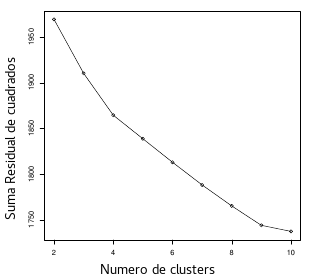
\includegraphics[width=0.7\textwidth]{Figuras/codo.png}
        \caption{Curva creada iterando valores de $K$ para la función $RSS_{min}(K)$}
        \label{fig:codo}
        \source{Imagen extraída de \cite{informationretrieval}}
      \end{figure}

    Un segundo tipo de criterio para cardinalidad de \textit{clusters} impone una penalidad por cada nuevo \textit{cluster}, conceptualmente se empieza con un unico \textit{cluster} que contiene todos los documentos y luego se busca el numero optimo de \textit{clusters} $K$ incrementando sucesivamente $K$ por uno. Esta función combina dos elementos, la distorcion que mide que tantos documentos se desvían del prototipo de sus \textit{clusters} ($RSS$ para K-medias); y una medida de complejidad de modelo. Se interpreta un agrupamiento como un modelo de los datos. La complejidad de modelo es agrupamiento es usualmente el numero de \textit{clusters} o una función para ello. Para el caso de K-medias, entonces se tiene como criterio para seleccionar $K$:
      \begin{equation} \label{eq:criterio2} 
        K = \arg_K \min[{RSS_{min}(K)+\lambda K}]
      \end{equation}

    donde $\lambda$ es un factor de ponderación. Un valor grande de $\lambda$ favorece una solución con pocos \textit{clusters}. Para $\lambda = 0$, no hay penalidad por mas \textit{clusters} y $K=N$ es la mejor solución.\cite{informationretrieval}

      


  \subsubsection{Clasificación jerárquica}
    La clasificación jerárquica no requiere la especificación de un numero de \textit{clusters} y la mayoría de los algoritmos utilizados para este tipo de clasificación son deterministicos. Estas ventajas vienen con el costo de una baja eficiencia.
    Los algoritmo de aficionan jerárquica los hay \textit{top-down}, donde requieren un método para dividir un \textit{cluster} de forma recursiva hasta que se alcancen los documentos individuales; y \textit{bottom-up}, donde cada documento es tratado como un cluster de un único elemento al principio, estos son luego mezclados (o aglomerados) en pares de forma sucesiva, este proceso se repite hasta que todos los \textit{clusters} sean mezclados en uno único que contenga todos los documentos, este algoritmo es conocido como HAC por sus siglas en ingles \textit{Hierarquical Aglomerative Clustering}.\cite{informationretrieval}   


    \paragraph{Dendogram}

      \begin{figure}[!htbp]
        \centering
        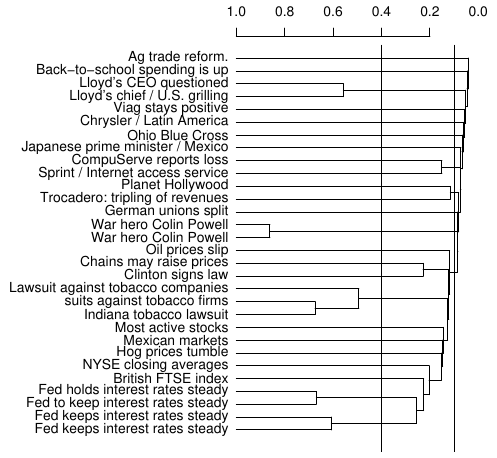
\includegraphics[width=0.7\textwidth]{Figuras/dendograma.png}
        \caption{Dendograma}
        \label{fig:dendograma}
        \source{Imagen extraída de \cite{informationretrieval}}
      \end{figure}

  

      Los agrupamientos HAC son generalmente visualizados en dendogramas, como se muestra en la figura \ref{fig:dendograma}. Cada mezcla esta representada por una linea horizontal, las coordenadas $y$ de esta linea es la similaridad de los dos \textit{clusters} que fueron unidos. Esta similitud es llamada similitud de la combinación del \textit{cluster} mezclado. El dendograma permite reconstruir la historia de las diferentes mezclas que se necesitaron para un agrupamiento especifico.\cite{informationretrieval}
    
      Para obtener un partición de \textit{clusters} diferenciados, como en el agrupamiento plano, la jerarquía debe ser cortada en algún punto. Pueden usarse diferente criterios para este fin: 

      \begin{itemize}
        \item Cortar en un nivel de similitud previamente especificado.
        \item Cortar el dendograma donde la distancia de similitud entre dos combinaciones sucesivas es mayor.
        \item  Aplicar la ecuación \ref{eq:criterio2}: 
            \begin{equation}\label{eq:criterio2.2}
               K = \arg_{K'} \min{[RSS(K')+\lambda K']}
            \end{equation} 

            Donde $K'$ se refiere al corte de la jerarquia que resulta en $K'$ \textit{clusters}, $RSS$ es la suma residual de cuadrados y $\lambda$ es una penalidad por cada \textit{cluster} adicional.
         \item También es posible especificar un numero $K$ de \textit{clusters} y seleccionar el corte que genere dicho numero.

      \end{itemize}

   


    \paragraph{Agrupamiento jerárquico simple}
      Primero se computa la matriz de similitud $C$, $N\times N$. El algoritmo luego ejecuta $N-1$ pasos de mezclar los \textit{clusters}actualmente mas similares. En cada iteración los dos \textit{clusters} mas similares son mezclados, y las filas y columnas del \textit{cluster} mezclado $i$ en $C$ son actualizadas.El agrupamiento es almacenado como una lista de mezclas en $A$. $I$ indica cuales \textit{clusters} estan disponibles para ser mezclados. La función $SIM(i,m,j)$ calcula la similaridad del cluster $j$ con la mezcla de los cluster $m$ e $i$. Este algoritmo sera refinado para las variantes de agrupamiento de enlace-individual, agrupamiento de enlace-completo, agrupamiento grupo-promedio y agrupamiento por centroide.\cite{informationretrieval}

 \begin{figure}[!htbp]
        \centering
        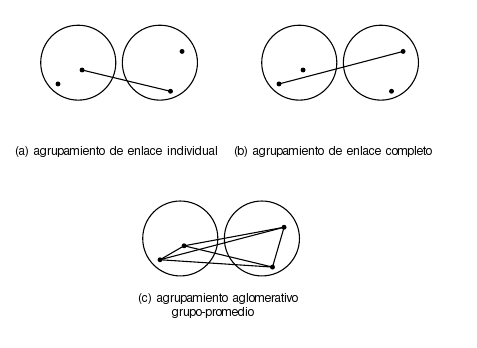
\includegraphics[width=0.7\textwidth]{Figuras/h_clust1.png}
        \caption{Tipos de agrupamientos jerarquicos}
        \label{fig:hclust}
        \source{Imagen extraída de \cite{informationretrieval}}
\end{figure}

\paragraph{Agrupamiento de enlace individual}
  En este agrupamiento la similaridad de dos \textit{clusters} es la similitud de sus miembros mas similares , ejemplo de esto se puede observar en la figura \ref{fig:hclust} (a). Este criterio es local, solo se toma en cuenta el área donde los dos \textit{clusters} están mas cercanos.\cite{informationretrieval}


\paragraph{Agrupamiento de enlace completo}

En el agrupamiento de enlace completo, la similitud de dos \textit{clusters} es la similitud de sus miembros menos similares, ejemplo en la figura \ref{fig:hclust} (b). Este criterio es no-local, la estructura completa del agrupamiento puede influenciar las decisiones al realizarse la mezcla. Esto resulta en una preferencia por \textit{clusters} compactos con diámetros pequeños, sobre \textit{clusters} largos y desordenados, sin embargo también causa sensibilidad ante valores atípicos.\cite{informationretrieval}

\paragraph{Agrupamiento aglomerativo grupo-promedio}
  El GAAC por sus siglas en ingles \textit{Group-average agglomerative clustering}, evalúa la calidad del \textit{cluster} basándose en la similitud entre todos los documentos, como se aprecia en la figura \ref{fig:hclust} (c). GAAC calcula la similitud promedio $SIM\mathrm{-}GA$ de todos los pares de documentos incluyendo pares del mismo \textit{cluster},excluyendo las similitudes de un elemento consigo mismo:

  \begin{equation}\label{eq:simga}
    SIM\mathrm{-}GA(\omega_i,\omega_j)=\frac{1}{(N_i+N_j)(N_i+N_j-1)}[(\sum_{d_m\in\omega_i\cup\omega_j}\vec{d_m})^2-(N_i+N_j)]
  \end{equation}

  donde $\vec{d}$ es la longitud normalizada del vector del documento $d$, $N_i$ y $N_j$ son el numero de documentos en $\omega_i$ y $\omega_j$, respectivamente.\cite{informationretrieval}
